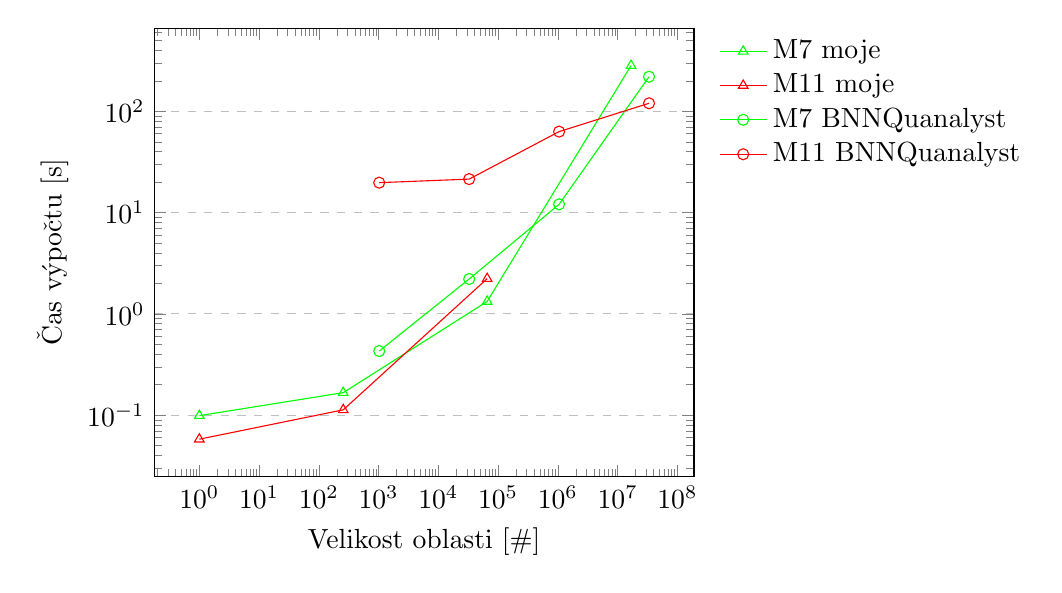
\begin{tikzpicture}
\begin{loglogaxis}[
    xlabel={Velikost oblasti [\#]},
    ylabel={Čas výpočtu [s]},
    legend pos=outer north east,
    legend style={draw=none, fill=none},
    legend cell align={left},
    ymajorgrids=true,
    grid style=dashed,
]

\addplot[
    color=green,
    mark=triangle,
    ]
    coordinates {
		(1, 0.099) (256, 0.167) (65566, 1.327) (16777216, 282.620)
    };

\addplot[
    color=red,
    mark=triangle,
    ]
    coordinates {
		(1, 0.058) (256, 0.113) (65566, 2.229)
    };

\addplot[
    color=green,
    mark=o,
    ]
    coordinates {
        (2^10, 0.43) (2^15, 2.21) (2^20, 12.07) (2^25, 219.4)
    };

\addplot[
    color=red,
    mark=o,
    ]
    coordinates {
        (2^10, 19.75) (2^15, 21.41) (2^20, 63.02) (2^25, 120.0)
    };

\legend{M7 moje, M11 moje, M7 BNNQuanalyst, M11 BNNQuanalyst}

\end{loglogaxis}
\end{tikzpicture}
